$y=e^{x/a}+e^{-x/a}$, $y=0$, $x=\pm a$

\nopagebreak
\begin{align*}
y = 2\cosh(x/a). \\
A &= \int_{-a}^{a} (e^{x/a} + e^{-x/a}) \, dx \\
&= \left[ a e^{x/a} - a e^{-x/a} \right]_{-a}^{a} \\
&= a (e^1 - e^{-1}) - a (e^{-1} - e^1) \\
&= a(e - 1/e) + a(e - 1/e) = 2a(e - 1/e) \\
&= 4a \sinh(1)
\end{align*}

\[
\boxed{\displaystyle 2a(e - e^{-1})}
\]

\begin{center}
    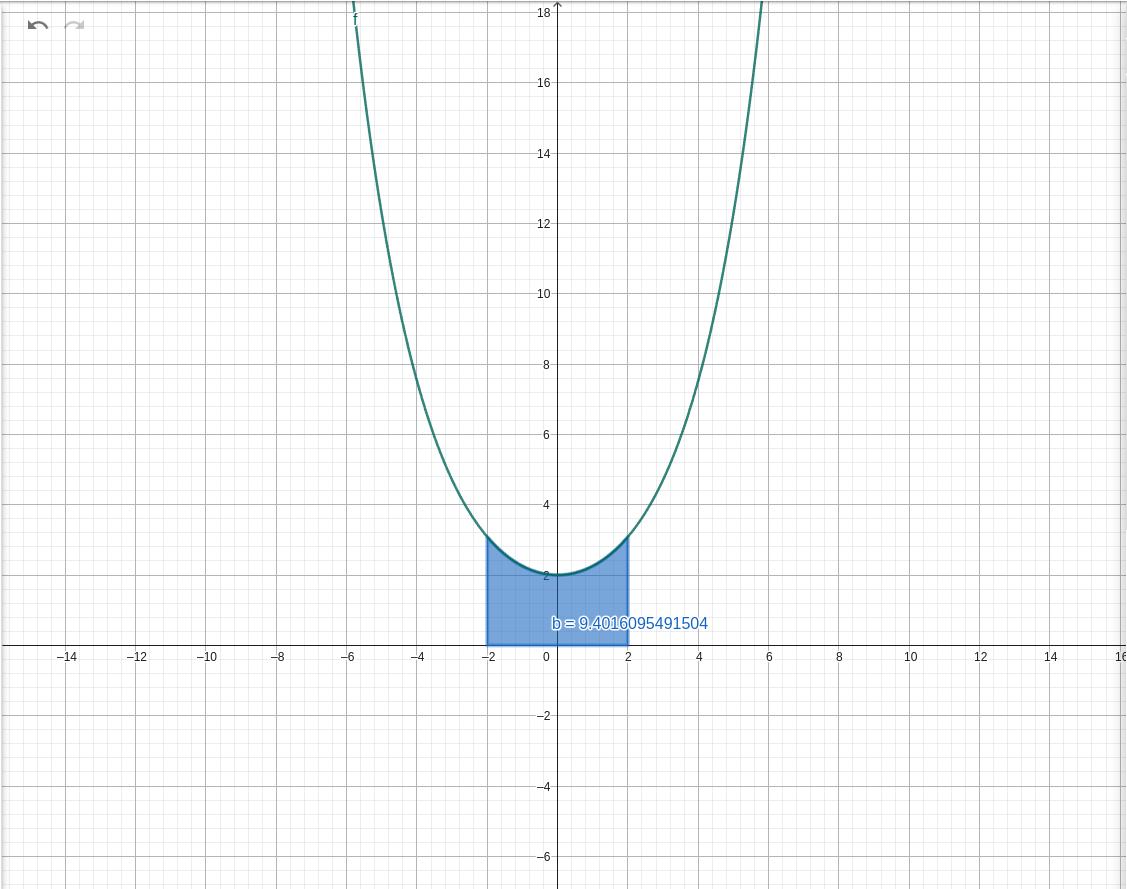
\includegraphics[width=0.5\textwidth]{Graficas/ejer23.png}
\end{center}
